%\documentclass[xcolor=dvipsnames]{beamer}
\documentclass[mathserif,10pt]{beamer}

\mode<presentation>
{
  \usetheme{UIUC}
} 

\newcommand{\cmt}[1]{}
\setbeamercovered{transparent=50}
\newcommand{\LIR}{{\tt LLVM IR}}
\newcommand{\MC}{{\tt Machine Code}}
\usepackage{listings}
\usepackage{amsmath}

\title[allvm]{allvm - Binary Decompilation}
\author{Sandeep Dasgupta}
\institute[UIUC]{University of Illinois Urbana Champaign}
\date{\today}


%if u want to show off the sections only
\setcounter{tocdepth}{1}

\lstset{language=[ANSI]C}
\lstset{% general command to set parameter(s)
  basicstyle=\footnotesize\tt, % print whole listing small
    identifierstyle=, % nothing happens
    commentstyle=\color{red}, % white comments
    showstringspaces=false, % no special string spaces
    lineskip=1pt,
    captionpos=b,
    frame=single,
    breaklines=true
      %\insertauthor[width={3cm},center,respectlinebreaks]
}



% If you want to come back to the subsection in outline everytime:
%\AtBeginSubsection
%{
%  \begin{frame}<beamer>{Outline}
%    \tableofcontents[currentsection,currentsubsection]
%  \end{frame}
%}

\AtBeginSection
{
  \begin{frame}<beamer>{Outline}
    \tableofcontents[currentsection,currentsubsection]
  \end{frame}
}


\begin{document}

\begin{frame}
\titlepage
\end{frame}


%%%%%%%%%%%%%%%%%%%%%%%%%%%%%%%%%%%%%%%%%%%%%%%%%%%%%%%%%%%%%%%%%%%%%%%%%%%%%%%%%%%%%
\section{Goal \& Motivation}
\subsection{Research Goal} %3:25 
\frame
{
  \frametitle{\subsecname}
  \begin{itemize}
    \item Research Goal
      \begin{itemize}
        \item Obtain ``richer'' LLVM IR than native machine code.
        \item Enable advanced compiler techniques ( e.g. pointer analysis, information flow tracking, automatic vectorization)
      \end{itemize}
  \end{itemize}

  \cmt{ 
    Today I will be presenting our work on binary dec ... 
      First I will start with the research goal which is to 
      obtain a richer version of llvm IR than the machine code 
      which entails more source level information (like variable , type , agregate structures,
       control flow,    ) than the native binary

      A related goal is that having such a  rich IR 
      we can do many sophisticated analyis, optimizations and code generation on them
      enable various compiler 
      analysis like pointer analysis, ...

      [Information flow in an information theoretical context is the transfer of information from a variable x to a variable y in a given process.
Not all flows may be desirable. For example, a system should not leak any secret (explicitly or implicitly) to public observers. ]

    /*
       Goal involves experimental understanding of the trade-offs between
      different approaches to reconstructing a richer IR.
      */

    why llvm ir: 
      sophisticated analysis, optimization, and code generation for code from arbitrary languages
             at arbitrary points in the lifetime of software. The diff points could be 
             compile time, link time, install time, load time, run-time,
           “idle-time” 
  }
}

\subsection{Why ``richer'' LLVM IR} 
\frame
{
  \frametitle{\subsecname}
   \begin{itemize}
      \item Source code analysis not possible
        \begin{itemize}
          \item IP-protected software 
          \item Malicious executables 
          \item Legacy executables
        \end{itemize}
      \item Source code analysis not sufficient
        \begin{itemize}
          \item What-you-see-is-not-what-you-execute
        \end{itemize}
      \item End-user security enforcement
      \item Platform aware optimizations
    \end{itemize}

  \cmt{ 
  Absence of source-code: There are several scenariojs where the original
source-code is not accessible. 
below: 
  - IP-protected software 
  - Third-party library and software components
  - Malicious executables 
  - Legacy executables 

  All such situations analysis of a HLIR is more beneficial than execuatble analyis
  For example, in case of IP protected sf or a known Malicious software, 
  in order to certify the behavior and uncover vulnerabilities HLIR analysis is 
  more benefial than exec analysis because the former contain HL source code semantics.  
    
    Also for legacy executable for which no 
    source code is avalailable aand running on outdated config.... executable 
    analysis is required which can recover functionally correct
      source-code components from such legacy software, so that such legacy
      systems can be ported to secure configurations. 

  even if we have the source code, exectatble analysis after 
  converting it to IR is more beneficial than source code analysis.

  Source-code analysis not sufficient
    There are several scenarios An executable code might demonstrate differ- ent behavior from
    the original source code. This phenomenon is popularly known as
    What-you-see-is-not-what-you-execute 
    Modifications can happen to the source code during compilation
    (optimizations) or after the compilation process (bad code injection).
    These modifications can significantly alter the program behavior. Con-
    sequently, the exact behavior of any program can only be uncovered by
    analyzing the executable code and the analysis of the exec is much more effective if
    done at the hihger level

    /*
       Moreover, several components of a typical software might be developed in
    multiple languages (Fortran, C and C++). 
    The analysis of the source code with diff lang is more diff
    that the analysis of the exec havinga consistent rep.
  */

  End-user security enforcement.: proposal pdf
  The software available to the end user is often in eec format w/o the source code
  and enforcing security features at that level is 
  difficult beciase of the absence of any semantic knowledge about the program,

  so extracting a high level IR is beneficial i this scenario

  Platform aware optimizations
    Binaries compiled for wide distribution are often targeted for one
    particular ISA and are rarely optimized for a particular processor.  Binary
    tools on an end-user platform can apply custom transforma- tions to take
    advantage of platform-specific information like exact knowledge of the
    memory hierarchy or the precise version of multimedia instructions.
  
  }
}

%%%%%%%%%%%%%%%%%%%%%%%%%%%%%%%%%%%%%%%%%%%%%%%%%%%%%%%%%%%%%%%%%%%%%%%%%%%%%%%%%%%%%
\section{Possible Approaches}
  \subsection{The 3 Possible Approaches} % 4:37 (+7.62)
  \frame
  {
    \frametitle{\subsecname}
    \begin{itemize}
      \item Decompile \MC \ $\rightarrow$ \LIR
        \begin{itemize}
          \item Easy to adopt
          \item No compiler support needed
        \end{itemize}
      \item ``Annotated'' \MC \ $\rightarrow$ \LIR
        \begin{itemize}
          \item Effective reconstruction of higher level IR
          \item Minimal compiler support needed
        \end{itemize}
      \item Ship \LIR
        \begin{itemize}
          \item Benefit:  \emph{No loss} of information via conversion to and from binary code.
        \end{itemize}
    \end{itemize}


    \cmt{
There are 3 possible approaches to achive the goal;
to <read> .. his is easy to adopt adn mos of the programstoday are shipped as native binaries
  also no extra compiler support is needed

  Seconf is to generate the binaru woth some annotations on it, which help help in
  recpnsruct the hogh kevel ir
  This requires compiler support but the goal here to to genetate minimal annotions
  which is sufficient to generate an high leve ir

  Thrisd is to ship ir directly; Obviously there will be no info loss

  As u can see all of them are having atradeoff between odoption and quality of llvm ir

    }

  }

  \subsection{Decompile \MC \ $\rightarrow$ \LIR}
  \frame
  {
    \frametitle{\subsecname}
    \begin{itemize}
      \item Challenge: Quality     
      \begin{itemize}
        \item Reconstructing code and control flow - much researched.
        \item Variable recovery
        \item Function \& ABI rules recovery
      \end{itemize}
    \end{itemize}

    \cmt{
        These methods make various trade-offs between ease of adoption, binary size,
        ease of shipping, and quality of the resulting LLVMIR, which directly
          affects the benefits that allvm provides.

          \item Diffrentiate data \& code.
          \item Indirect branch/call.
          \item Variable instruction size
          \item Position independent code (PIC) sequences
          \item Hand crafted assembly code

    This point is very well researched and exists varisus tools QEMU[8], BAP [7], Dagger [6], and Fracture [23].
    }


  }


  \subsection{``Annotated'' \MC \ $\rightarrow$ \LIR}
  \frame
  {
    \frametitle{\subsecname}
    \begin{itemize}
      \item Challenge: 
        \begin{itemize}
          \item Annotations must be ``minimal'' \& sufficient
          \item Annotations must be compiler and IR-independent
          \item Adoption
        \end{itemize}
    \end{itemize}

\cmt{ Another challenge is that the annotations should be compiler- and
  IR-independent, e.g., a non-LLVM commercial compiler such as Windows Visual
    C++ or Intel’s ICC should be able to produce them 

    what is the minimal information sufficient to reconstruct LLVM IR, so that
    redundant information is not encoded. A third question is how to encode the
    information compactly on native code, so that it does not blow up the size
    of executables.  1.2.3
    
    * Add another bullet
    here saying that we will learn from our experience with the first approach
    before we decide what the annotations need to be
}

  }

  \subsection{Ship \LIR}
  \frame
  {
    \frametitle{\subsecname}
    \begin{itemize}
      \item Challenge:
        \begin{itemize}
          \item Adoption in Non LLVM based compilers
          \item Stable distribution format for shipping  
          \item Risks to intellectual property
          \item Code size bloat
        \end{itemize}
    \end{itemize}
\cmt{

  There are compilers that do not use LLVM IR as an internal representation.

    The best solution for such compilers would be to treat LLVM IR as a target
    for producing code, such as the Dragonegg plugin that takes code compiled
      by GCC and converts it to LLVM IR instead. 
      
        LLVM IR is a relatively simple, orthogonal instruction set with
        an unlimited number of registers and targeting LLVM IR should be much
        easier than a back end for a native hardware architecture. 
        

        LLVMIR is not a fully frozen and stable ABI
     However, two commercial projects – Portable
     Native Client and Renderscript – are already shipping LLVM IR in modified
     form, so it is not an insurmountable barrier. 
     

     many commercial Java and .NET applications are shipped in rich bytecode
     languages (JVM or MSIL) that reveal extensive source-level semantic
     information. The way they reduce the risk to their intellectual property
     is to use deliberate obfuscation tools, e.g., ProGuard or DexGuard, which
     are far more effective than relying on standard binary code to prevent
     reverse engineering. If such tools can protect applications shipped in
     relatively high-level representations like JVM or MSIL, the techniques
     they use could be applied equally effectively to LLVM bitcode as well.
        
** Note: "Ship LLVM IR with machine code" already exists!  But requires source code and an LLVM-based compiler
  }
}

%%%%%%%%%%%%%%%%%%%%%%%%%%%%%%%%%%%%%%%%%%%%%%%%%%%%%%%%%%%%%%%%%%%%%%%%%%%%%%%%%%%%%%
\section{Our Approach}
  \subsection*{Our Approach}
  \frame
  {
    \frametitle{\subsecname}
    \begin{itemize}
      \item Long term goal
        \begin{itemize}
          \item Minimal compiler-independent annotations to reconstruct high-quality IR
        \end{itemize}    
      \item Short term goals
        \begin{enumerate}
          \item Experiment with \MC\ $\rightarrow$ \LIR, to \textbf{understand} the challenges better
            \begin{itemize}
              \item To select an existing decompilation framework.
              \item Experiment with different variable and type recovery strategies
            \end{itemize}    
          \item Design suitable annotations for what cannot be inferred without them
        \end{enumerate}    
    \end{itemize}

      \cmt{

** Note: "Ship LLVM IR with machine code" already exists!  But requires source code and an LLVM-based compiler
      }


  }


\section{Decompile \MC \ $\rightarrow$ \LIR}
  \subsection{Variable \& Function Parameter Recovery}
  \frame
  {
    \frametitle{\subsecname}
    \begin{itemize}
      \item Benefit
        \begin{itemize}
          \item Enables many fundamental analysis (Dependence, Pointer analysis)
          \item Functional IR
        \end{itemize}
      \item State of the art
        \begin{itemize}
          \item Divine
            \begin{itemize}
              \item State of the art variable recovery %Not scalable 
            \end{itemize}     
          \item Second Write 
            \begin{itemize}
              \item Heuristics for function parameter  detection
              \item Scalable variable and type recovery
            \end{itemize}     
          \item TIE %(Type Inference On Execuatbles)
            \begin{itemize}
              \item Type recovery
            \end{itemize}     
        \end{itemize}
    \end{itemize}

    \cmt{
      Not scalable
    }

  }


\section{mcsema}
  \subsection{Choosing mcsema}
  \frame
  {
    \frametitle{\subsecname}
    \begin{itemize}
      \item Functional \LIR
      \item Separation of modules: CFG recovery and CFG $\rightarrow$ \LIR
      \item Actively supported and open sourced
    \end{itemize}

    \begin{figure}[h]
      \centering
        \scalebox{0.45}{
          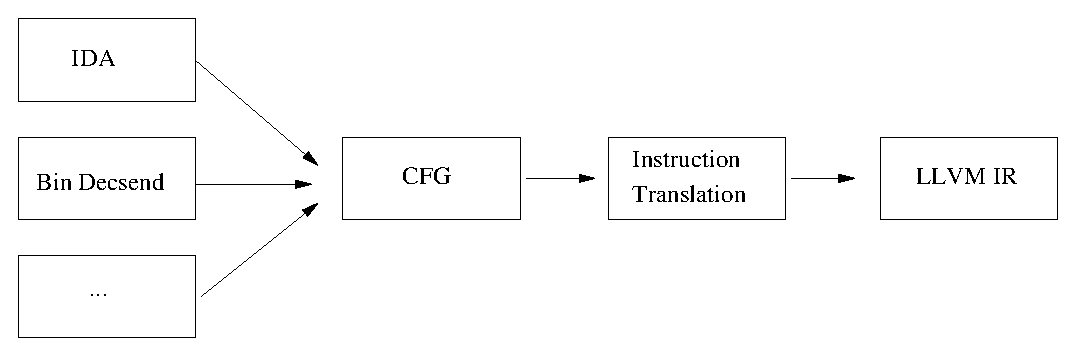
\includegraphics{Figs/1.eps}
        }
    \end{figure}
  }

  \subsection{Support \& Limitations}
  \frame
  {
    \frametitle{\subsecname}
    \begin{itemize}
      \item What Works
        \begin{itemize}
          \item Integer Instructions
          \item FPU and SSE registers
          \item Callbacks, External Call, Jump tables 
        \end{itemize}
      \item In Progress
        \begin{itemize}
          \item FPU and SSE Instructions: Not fully supported
          \item Exceptions
          \item Better Optimizations
        \end{itemize}
    \end{itemize}
  }

\section{Demo}
  \subsection{mcsema: Demo}
  \frame
  {
    \frametitle{\subsecname}
  }

\section{Backup} 
  \subsection{What-you-see-is-not-what-you-execute} 
  \frame
  {
    \frametitle{\subsecname} 
    The following compiler (Microsoft C++ .NET) induced vulnerability was discovered
               during the Windows security push in 2002
    \begin{figure}[h]
      \centering
        \scalebox{0.75}{
          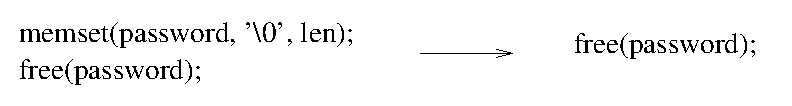
\includegraphics{Figs/2.eps}
        }
    \end{figure}
    %\cmt{
     %          fragment shown in the following on the left never uses the
     %          values written by memset (intended to scrub the buffer pointed
      %%             to by password), the memset call could be removed, thereby
      %         leaving sensitive information exposed in the freelist at
      %         runtime.  
      %         
      %         memset(password, �\0�, len); free(password); =�
      %         free(password); 
    %}
  }




















\end{document}


